\documentclass[oneside]{abntex2-unisul}

\usepackage{lipsum} % para geração de dummy text
\usepackage{tikz} % graficos
\usepackage{pgfplots} % graficos

% glossarios extras
\newglossary[abb.alg]{abbrev}{abb.acr}{abb.acn}{Abreviaturas}
% prepara os glossarios
\makeglossaries

\titulo{<O Título do Seu Trabalho Aqui>}
\autor{<Nome Aluno 1>\\ <Nome Aluno 2>}
\local{<Cidade>}
\data{<Ano de Publicação>}

\orientador[Orientador:]{<Nome do(a) Orientador(a)>}
\coorientador[Coorientador:]{<Nome do(a) Coorientador(a)>}

\instituicao{Universidade do Sul de Santa Catarina}
\tipotrabalho{Trabalho de Conclusão de Curso}

\naturezatrabalho{Este Trabalho de Conclusão de Curso foi julgado adequado à obtenção do título de... <Bacharel, Licenciado, Mestre, Especialização ou Tecnólogo> em... <área de concentração> e aprovado em sua forma final pelo Curso de... <nome do curso>, da \imprimirinstituicao.}
\preambulo{Trabalho de Conclusão de Curso apresentado ao Curso de <graduação, pós-graduação ou tecnólogo> em... <nome do curso>, da \imprimirinstituicao, como requisito parcial para obtenção do título de.. <Bacharel, Licenciado, Mestre, Especialização ou Tecnólogo>.}

\membrobancaA[\imprimirinstituicao]{Prof. e orientador \imprimirorientador}
\membrobancaB[Universidade B]{Membro B}
\membrobancaC[Universidade C]{Membro C}

% cadastro glossarios e acronimos
%!TEX root = tcc.tex

\newglossaryentry{dissertacao}{
  name=Dissertação,
  text=dissertação,
  description={Uma modalidade de redação ou composição, escrita em prosa ou apresentada de forma oral}}

%!TEX root = tcc.tex

\newdualentry{sc}{SC}{Santa Catarina}{Uma das 27 unidades federativas do Brasil, localizada no centro da região Sul do país}
%!TEX root = tcc.tex

\newglossaryentry{sum}{
  type=symbols,
  name={Somatória},
  text={somatória},
  symbol={\ensuremath{\sum}},
  description={- \emph{Summation} - Soma de todos os valores no invervalo}}
%!TEX root = tcc.tex

\newdualentry[][type=abbrev]{unisul}{UNISUL}{Universidade do Sul de Santa Catarina}{Fundação criada pelo poder municipal de Tubaração-SC, em operação do sul ao norte do estado de Santa Catarina}

\begin{document}

    % Elementos pré-textuais
    \pdfbookmark[0]{Capa}{capa}
    \pretextual
    \imprimircapa
    \imprimirfolhaderosto{}
    %!TEX root = tcc.tex

\begin{errata}
Errata!
\end{errata}

    \imprimirfolhadeaprovacao
    %!TEX root = tcc.tex

\begin{dedicatoria}
Texto das dedicatórias. Texto das dedicatórias. Texto das dedicatórias. Texto das dedicatórias. Texto das dedicatórias. Texto das dedicatórias. Texto das dedicatórias. Texto das dedicatórias. Texto das dedicatórias.
\end{dedicatoria}
    %!TEX root = tcc.tex

\begin{agradecimentos}

\lipsum[1]

\end{agradecimentos}
    \begin{epigrafe}
"Epígrafe epígrafe epígrafe epígrafe epígrafe epígrafe epígrafe epígrafe epígrafe epígrafe epígrafe epígrafe epígrafe epígrafe epígrafe." (AUTOR, ano)
\end{epigrafe}
    \begin{resumo}

Lorem ipsum dolor sit amet, consectetur adipiscing elit. Suspendisse adipiscing eu libero non ultricies. Donec accumsan, turpis ut malesuada facilisis, felis augue porta quam, et lacinia turpis ligula et risus. Suspendisse lobortis ipsum ligula, ut accumsan tortor tempus lacinia. Praesent eu nisi vehicula, cursus ipsum vel, suscipit nulla. Mauris fringilla ullamcorper orci eu ullamcorper. Praesent eget tristique magna. Nulla varius libero placerat, viverra nisi volutpat, iaculis leo. Nullam vel metus in nunc fringilla tristique vel ut tortor.
\\\\
\noindent
Palavras-chave: latex. abntex. editoração de texto.

\end{resumo}
    \begin{resumo}[Abstract]
\begin{otherlanguage*}{english}

Fusce tempor nec est eu tincidunt. Aenean consectetur accumsan quam non aliquam. Vestibulum ac hendrerit massa. Aliquam dictum lacinia ullamcorper. Phasellus posuere nunc nec felis vulputate, non facilisis metus aliquet. Aenean faucibus, lacus et congue tristique, mi turpis faucibus mi, sed rhoncus nibh erat sed lorem. Vivamus erat nunc, eleifend id lorem in, euismod tempus sem.
\\\\
\noindent
Key-words: latex. abntex. text editoration.

\end{otherlanguage*}
\end{resumo}
    \pdfbookmark[0]{\listfigurename}{listoffigures}
    \listoffigures*
    \clearpage
    \pdfbookmark[0]{\listtablename}{listoftables}
    \listoftables*
    \clearpage
    \pdfbookmark[0]{Abreviaturas}{abreviaturas}
    \printacronyms[type=abbrev] % abreviaturas
    \clearpage
    \pdfbookmark[0]{\acronymname}{printacronyms}
    \printacronyms % siglas
    \clearpage
    \pdfbookmark[0]{\glssymbolsgroupname}{printsymbols}
    \printsymbols[style=symbol] % simbolos
    \clearpage
    \pdfbookmark[0]{\contentsname}{tableofcontents}
    \tableofcontents*
    \cleardoublepage

    % Elementos textuais
    \textual
    %!TEX root = tcc.tex
\chapter{Introdução} \label{ch:introducao}

\lipsum[1]

\lipsum[2]

\lipsum[3]

\section{Apresentação do problema}

\lipsum[1]

\section{Objetivos} \label{sec:obj}

\lipsum[1]

\subsection{Geral} \label{subsec:obj-general}

\lipsum[1]

\subsection{Específicos} \label{subsec:obj-spec}

\begin{enumerate}
  \item Pellentesque habitant morbi tristique senectus
  \item Phasellus eu tellus sit amet tortor gravida placerat
\end{enumerate}

\section{Justificativa}

\lipsum[1]

\section{Estrutura do trabalho}

Esse trabalho está dividido em 5 capítulos. O \cref{ch:introducao} traz
aspectos introdutórios, para compreender problemas relacionados e os objetivos, seguindo para uma solução que será detalhada nos capítulos posteriores.

O \cref{ch:rev-biliografica} apresenta os conceitos, técnicas utilizadas no desenvolvimento do trabalho.

O \cref{ch:solucao} apresenta a solução desenvolvida.

O \cref{ch:aplicacao} apresenta os resultados coletados com a aplidação da solução.

No \cref{ch:conclusao} é apresentada a conclusão do trabalho baseando-se nos resultados conquistados ao longo da pesquisa e desenvolvimento.


    \chapter{Cap. 2}

\lipsum
    %!TEX root = tcc.tex

\chapter{Solução} \label{ch:solucao}

\section{Figuras} \label{sec:figuras}

A \cref{fig:logo-unisul} apresenta o logo da UNISUL.

\begin{figure}[H]
\centering
\caption{Logo da Unisul}
\label{fig:logo-unisul}

\includegraphics[width=90mm]{logo_unisul}
\caption*{Fonte: http://unisul.br/}
\end{figure}

\lipsum[1]

\section{Tabelas} \label{sec:tabelas}

A \cref{tab:taxa-desemprego} apresenta a taxa de desemprego aberto.

\begin{table}[H]
\centering
\caption{Taxa de desemprego aberto, por região metropolitana, do primeiro semestre de 1992.}
\label{tab:taxa-desemprego}
\begin{tabular}{|c|c|c|c|c|}
\hline
\multirow{2}{*}{Ano e mês} & \multicolumn{4}{|c|}{Região metropolitana}          \\ \cline{2-5}
                           & Recife & Salvador & Belo Horizonte & Rio de Janeiro \\ \hline
Janeiro                    & 6.10   & 5.43     & 4.77           & 4.24           \\ \hline
Fevereiro                  & 6.44   & 5.18     & 5.00           & 3.81           \\ \hline
Março                      & 6.33   & 5.76     & 5.06           & 4.24           \\ \hline
Abril                      & 6.67   & 6.06     & 4.47           & 4.13           \\ \hline
Maio                       & 6.21   & 7.26     & 4.61           & 5.54           \\ \hline
Junho                      & 5.30   & 6.43     & 4.31           & 3.63           \\ \hline
\end{tabular}
\caption*{Fonte: FUNDAÇÃO INSTITUTO BRASILEIRO DE GEOGRAFIA E ESTATÍSTICA. \textbf{Normas de apresentação tabular}. 3.ed. Rio de Janeiro, 1993. p. 51}
\end{table}

\lipsum[1]

\section{Gráficos} \label{sec:graficos}

\begin{figure}[H]
  \centering
  \caption{Representação gráfica da \cref{tab:taxa-desemprego}}
  \label{fig:taxa-desemprego}
  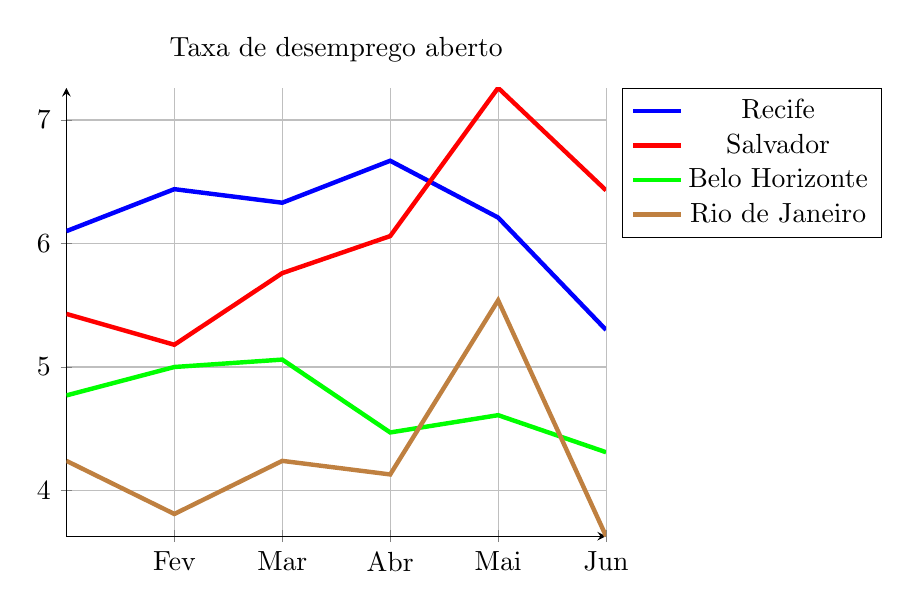
\begin{tikzpicture}
    \begin{axis}[
        grid=both,
        axis lines=middle,
        legend pos=outer north east,
        symbolic x coords={Jan, Fev, Mar, Abr, Mai, Jun},
        title={Taxa de desemprego aberto}
      ]
      \addplot[blue, ultra thick]
         coordinates{(Jan, 6.10)(Fev, 6.44)(Mar, 6.33)(Abr, 6.67)(Mai, 6.21)(Jun, 5.30)};
      \addlegendentry{Recife}
      \addplot[red, ultra thick]
         coordinates{(Jan, 5.43)(Fev, 5.18)(Mar, 5.76)(Abr, 6.06)(Mai, 7.26)(Jun, 6.43)};
      \addlegendentry{Salvador}
      \addplot[green, ultra thick]
         coordinates{(Jan, 4.77)(Fev, 5.00)(Mar, 5.06)(Abr, 4.47)(Mai, 4.61)(Jun, 4.31)};
      \addlegendentry{Belo Horizonte}
      \addplot[brown, ultra thick]
         coordinates{(Jan, 4.24)(Fev, 3.81)(Mar, 4.24)(Abr, 4.13)(Mai, 5.54)(Jun, 3.63)};
      \addlegendentry{Rio de Janeiro}
    \end{axis}
  \end{tikzpicture}
  \caption*{Fonte: Autor do Trabalho}
\end{figure}

\lipsum[1]

\section{Códigos} \label{sec:codigos}

\begin{figure}[H]
  \caption{Exemplo de JSON de retweet com números utilizados}
  \label{fig:retweet-json-numbers}
  \lstinputlisting[language=json, firstline=2, lastline=14]{code/retweet-sample-numbers.json}
  \caption*{Fonte: Autor do Trabalho}
\end{figure}

\lipsum[1]

\section{\emph{Glossaries}} \label{sec:glossaries}

Utilizando abreviatura pela primeira vez \gls{unisul}. Utilizando abreviatura pela segunda vez \gls{unisul}.

Utilizando sigla pela primeira vez \gls{sc}. Utilizando sigla pela segunda vez \gls{sc}.

Utilizando glossário pela primeira vez \gls{dissertacao}. Utilizando glossário pela segunda vez \gls{dissertacao}.

Utilizando simbolo pela primeira vez \glssymbol{sum}. Utilizando simbolo pela segunda vez \glssymbol{sum} \cite{latex-guide}. Abaixo equação com \gls{sum}:

$$
  \glssymbol{sum}_{i=0}(x+i)
$$

\section{Demais Referências} \label{sec:demais-ref}

A \cref{sec:figuras} apresentou como as figuras são utilizadas. A \cref{subsec:obj-general} apresentou o objetivo geral conforme \citeonline{latex-guide}.

    \chapter{Cap. 4}

\lipsum
    \chapter{Cap. 4}

\lipsum

    % Elementos pós-textuais
    \postextual
    \bibliography{tcc}
    \printglossary
    \addcontentsline{toc}{chapter}{\uppercase{\glossarytoctitle}}
    \apendices

\chapter{Primeiro apêndice}
Primeiro apêndice!

\chapter{Segundo apêndice}
Segundo apêndice
    %!TEX root = tcc.tex

\anexos

\chapter{Primeiro anexo}
Primeiro anexo!

\chapter{Segundo anexo}
Segundo anexo!

\end{document}